\documentclass[12pt]{exam}

\usepackage{amssymb}
\usepackage{mathtools}
\usepackage{algorithm}
\usepackage{float}  % Figure placement
\usepackage{minted}  % Code highlighting
\usepackage{tikz}  % Flow chart
\usepackage{lipsum}
\usepackage{xspace}
\usepackage{hyperref}
\usepackage{MnSymbol}
\usepackage{pgffor}
\usepackage{graphicx}
\usepackage{pdfpages}
\usepackage{listings}
\usepackage{caption}


\hypersetup{
    colorlinks = true,
    linkcolor = blue,
    urlcolor  = blue,
    citecolor = blue,
    anchorcolor = blue
}
\lstset{
  language=Python,
  breaklines=true,  % Enable line breaking
  basicstyle=\small % Reduce the size of the font
}

\newcommand{\hwheaderfooter}[3]{
\pagestyle{headandfoot}
\firstpageheadrule
\firstpageheader{#1}{#2}{#3}
\runningheader{#1}{#2}{#3}
\runningheadrule
\firstpagefooter{}{\thepage}{}
\runningfooter{}{\thepage}{}
}

\newcommand{\latex}{\LaTeX\xspace}

\newcommand{\stars}[1]{%
    \foreach \n in {1,...,#1}{%
        $\filledstar$%
    }%
}

\usetikzlibrary{shapes.geometric, arrows}
\tikzstyle{arrow} = [thick,->,>=stealth]

\hwheaderfooter{Project 1 - Maze}{Ching}{CSCI 406}


\begin{document}

\section*{Space Wreck Maze Problem}
The space wreck maze problem has the basic following rules:

\begin{itemize}
    \item The game has two players, Captain Rocket and Lieutenant Lucky.
    \item Each turn one player can move through a corridor to an adjacent room.
    \item The players can only move through corridors that are the same color as the room the other player is in.
    \item The game ends when either player reaches the goal room.
\end{itemize}


\begin{figure}[H]
    \centering
    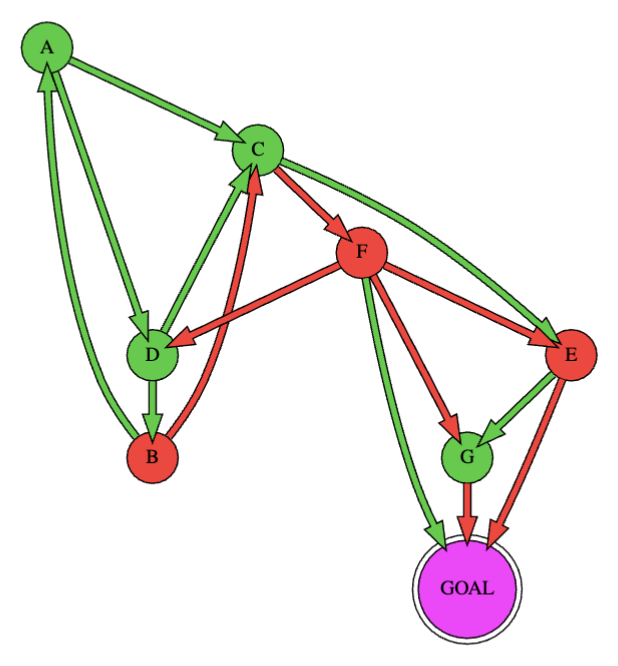
\includegraphics[width=0.5\textwidth]{board_graph.png}
    \caption{Sample Board Game (A=1,B=2...Goal=8)}
    \label{fig:board_graph}
\end{figure}

\noindent \textit{Refer to Appendix A for the full problem description.}


\section*{Graph Model}

To determine the shortest path of moves for the SpaceWreck puzzle game, a Breadth-First Search (BFS) algorithm was applied to a graph of game states. The input file, containing room and corridor colors, served as the basis for generating the game state graph. A representative snapshot of the game state graph is depicted in Figure \ref{fig:game_state_graph}.

\subsection*{Nodes}
The nodes in the game state graph correspond to each conceivable configuration of the game, identified by a tuple representing the room locations of Captain Rocket and Lieutenant Lucky. Figure \ref{fig:game_state_graph} provides a visual representation of this graph.

\subsection*{Edges}
The directed edges connecting nodes signify possible moves between game states. Each edge is labeled with the corresponding move required for the transition, denoting the player (Rocket or Lucky) and the new room number.

\subsection*{Special Features}
To allow for an unmodified BFS search (i.e. one start vertex and one end vertex), a single node was generated to represent the end game state. When generating the explicit graph, any edge that would result in a single player in the goal room was connected to this single end node, represented at $(n,n)$ on the state graph. This allows for a unmodified BFS search to be conducted from any game state node, representing the start, to the single goal state. Otherwise BFS must be modified to account for the $2n-1$ unique end game states.

The explicit representation of game states and moves provides a comprehensive model for applying BFS to find the shortest path in the SpaceWreck puzzle game.


\begin{figure}[H]
    \centering
    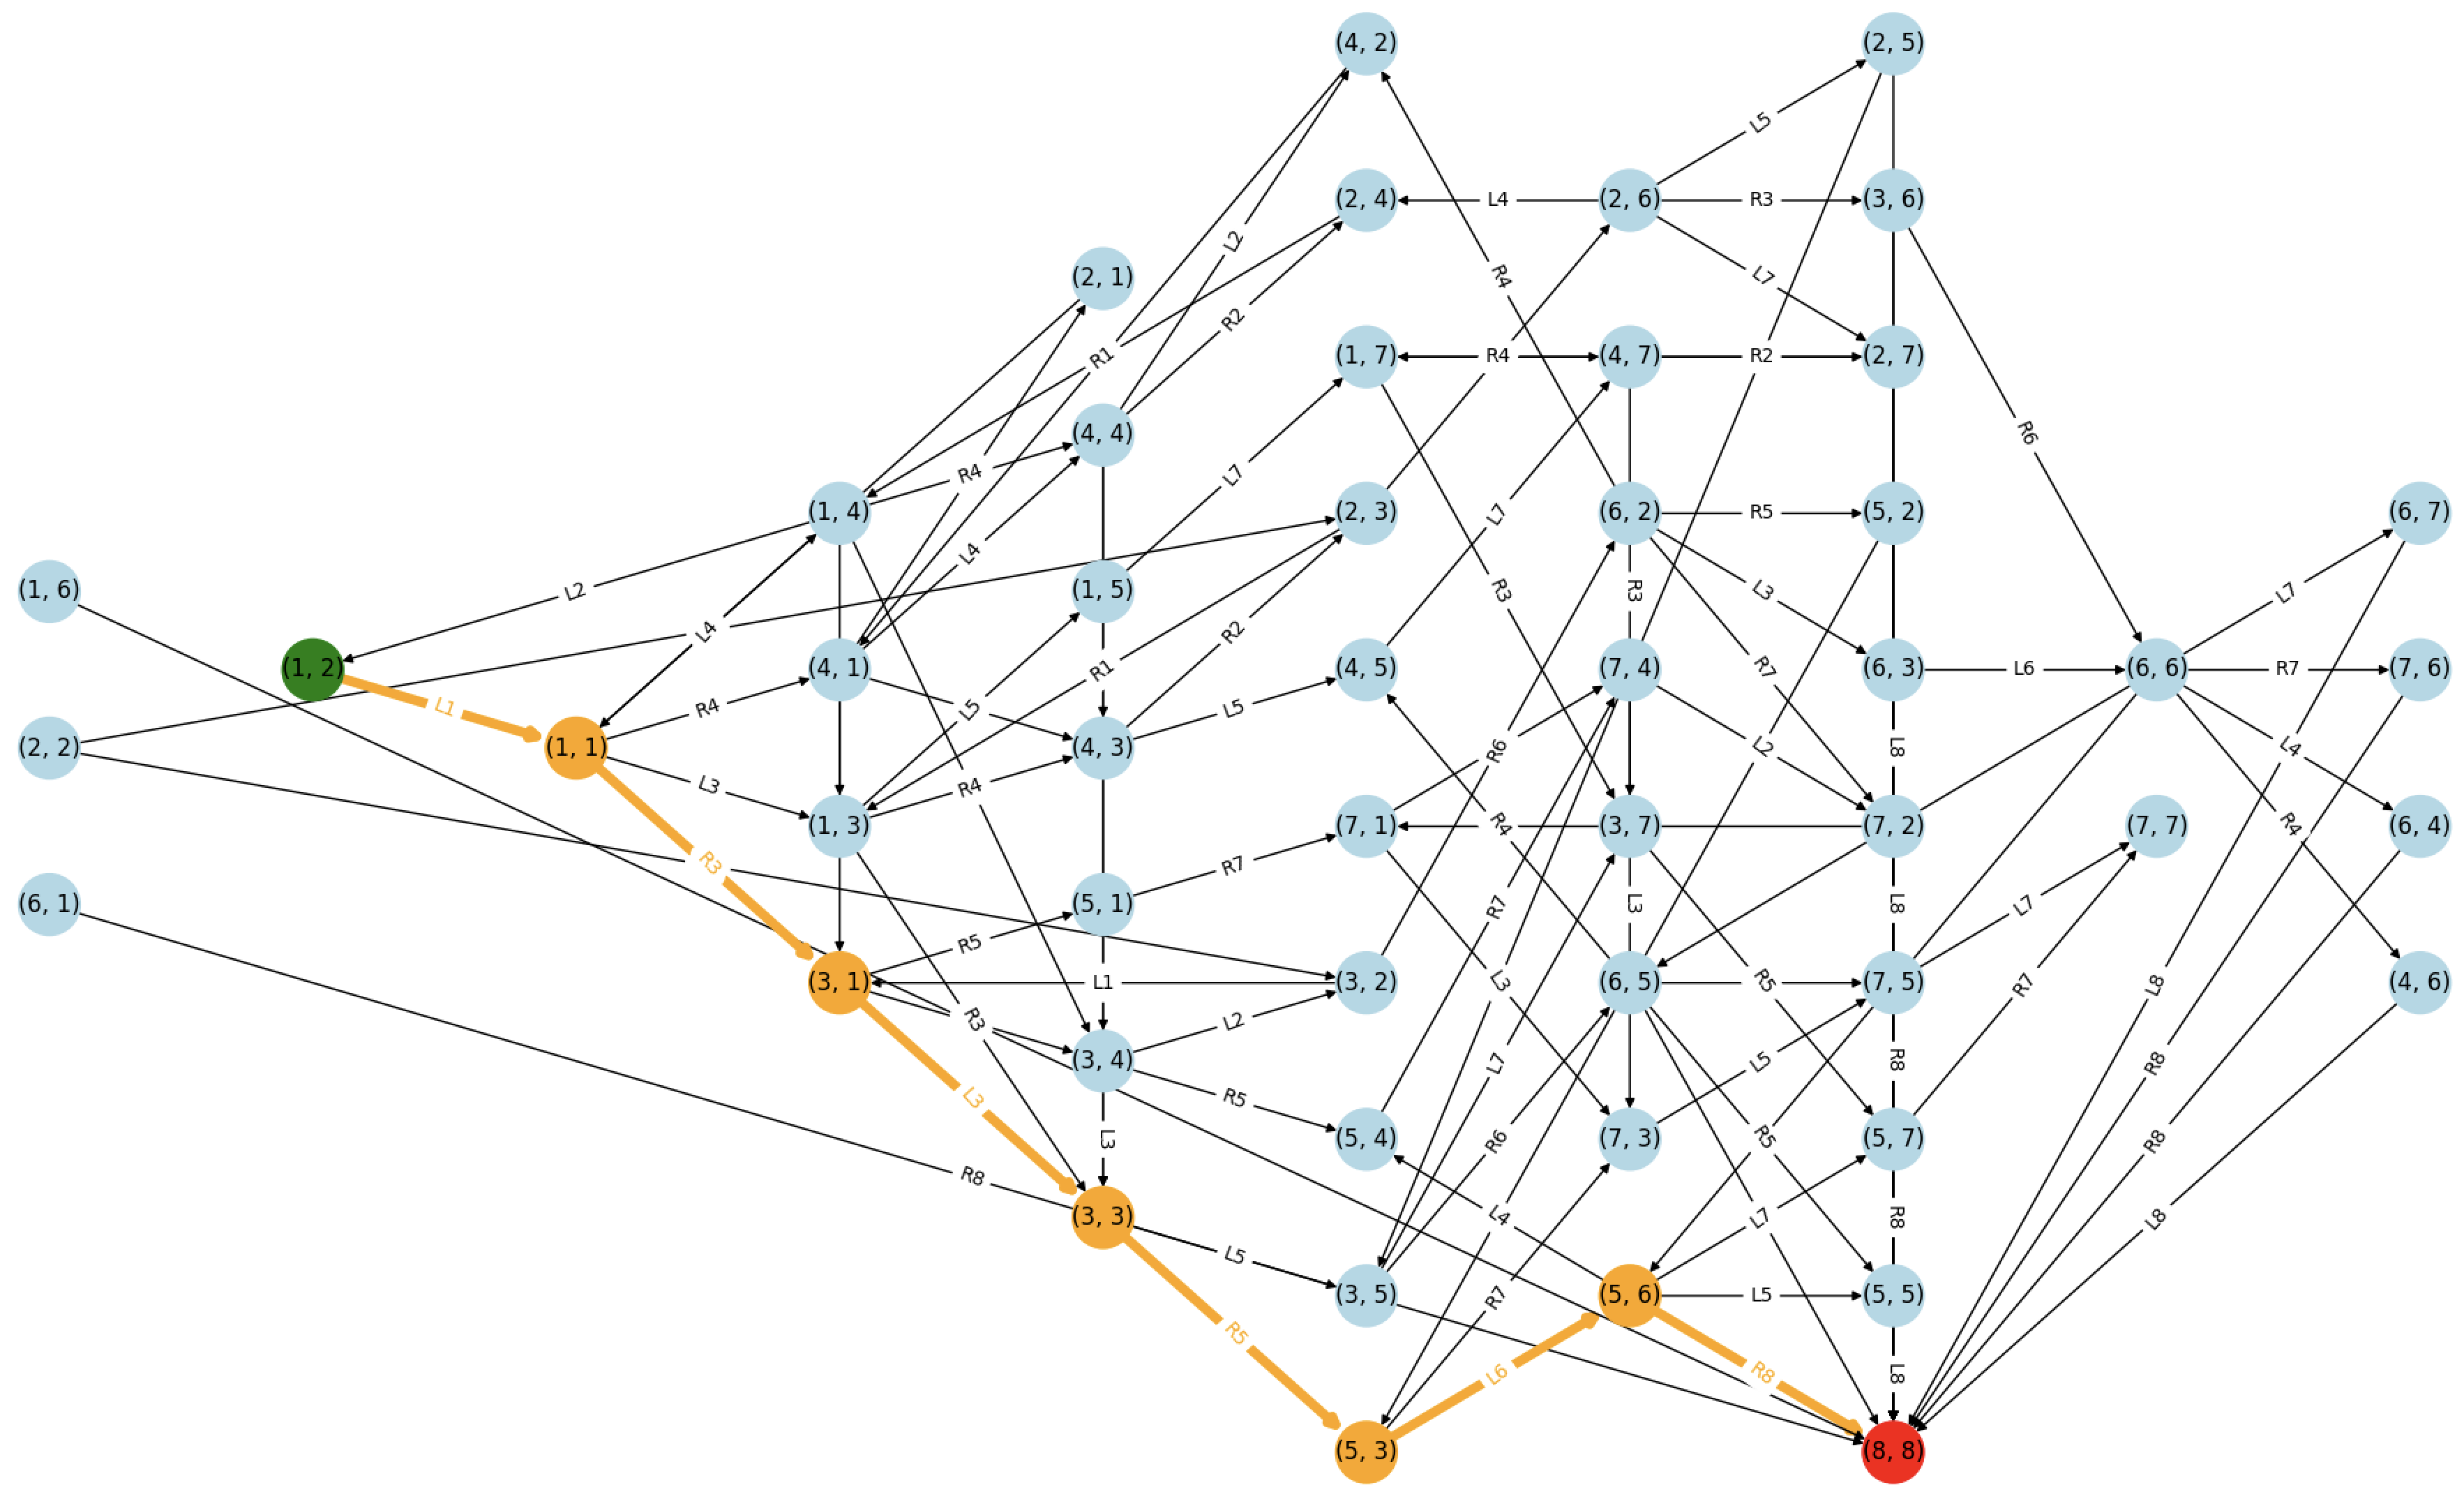
\includegraphics[width=\textwidth]{game_state_graph.png}
    \caption{Game State Graph (green=start node, red=end node, orange=shortest path)}
    \label{fig:game_state_graph}
\end{figure}


\section*{Model Accuracy}

As discussed in the graph model section, each vertex on the game state graph represents a distinct configuration of the SpaceWreck puzzle. The edges between vertices correspond to valid moves between game states. Being a directed graph, if you select any vertex any children of that vertex are the valid moves from that game state.

As this graph is explicitly defined and represented the whole game state space, it is guaranteed to contain all possible configurations and moves within the maze. This ensures that every potential solution path is represented in the graph.

BFS was chosen as the search algorithm due to its ability to systematically explore the graph, starting from the initial game state and traversing through subsequent states level by level. BFS is guaranteed to find the shortest path, if one exist, when a directed graph has a finite branching factor and finite depth. This is the case for the SpaceWreck maze game state graph.


\section*{Space Complexity}
Assume a maze of $n$ rooms and $m$ corridors.

The total size of the generated game state graph is $(n-1)^2 + 1$ vertices\footnote{the total number of nodes would be $n^2$ if the end node was not modeled as a singular node}. The graph is initialized by generating a node for every possible combination of room locations for rocket and lucky, $(1...n-1,1...n-1)$ and a single room of $(n,n)$ is generated representing all possible game states which result in the end of the game.

The maximum number of edges in the state graph is $\frac{v(v-1)}{2}$, where $v=(n-1)^2 + 1$, which occurs when the state graph is fully connected. This is because each node has the potential to connect to every other node, except for itself. This results in the upper bound of $O(v^2)$ edges or $O(n^4)$ edges.


\pagebreak
\section{Appendix A: Space Wreck Problem Description}
\begin{figure}[H]
    \centering
    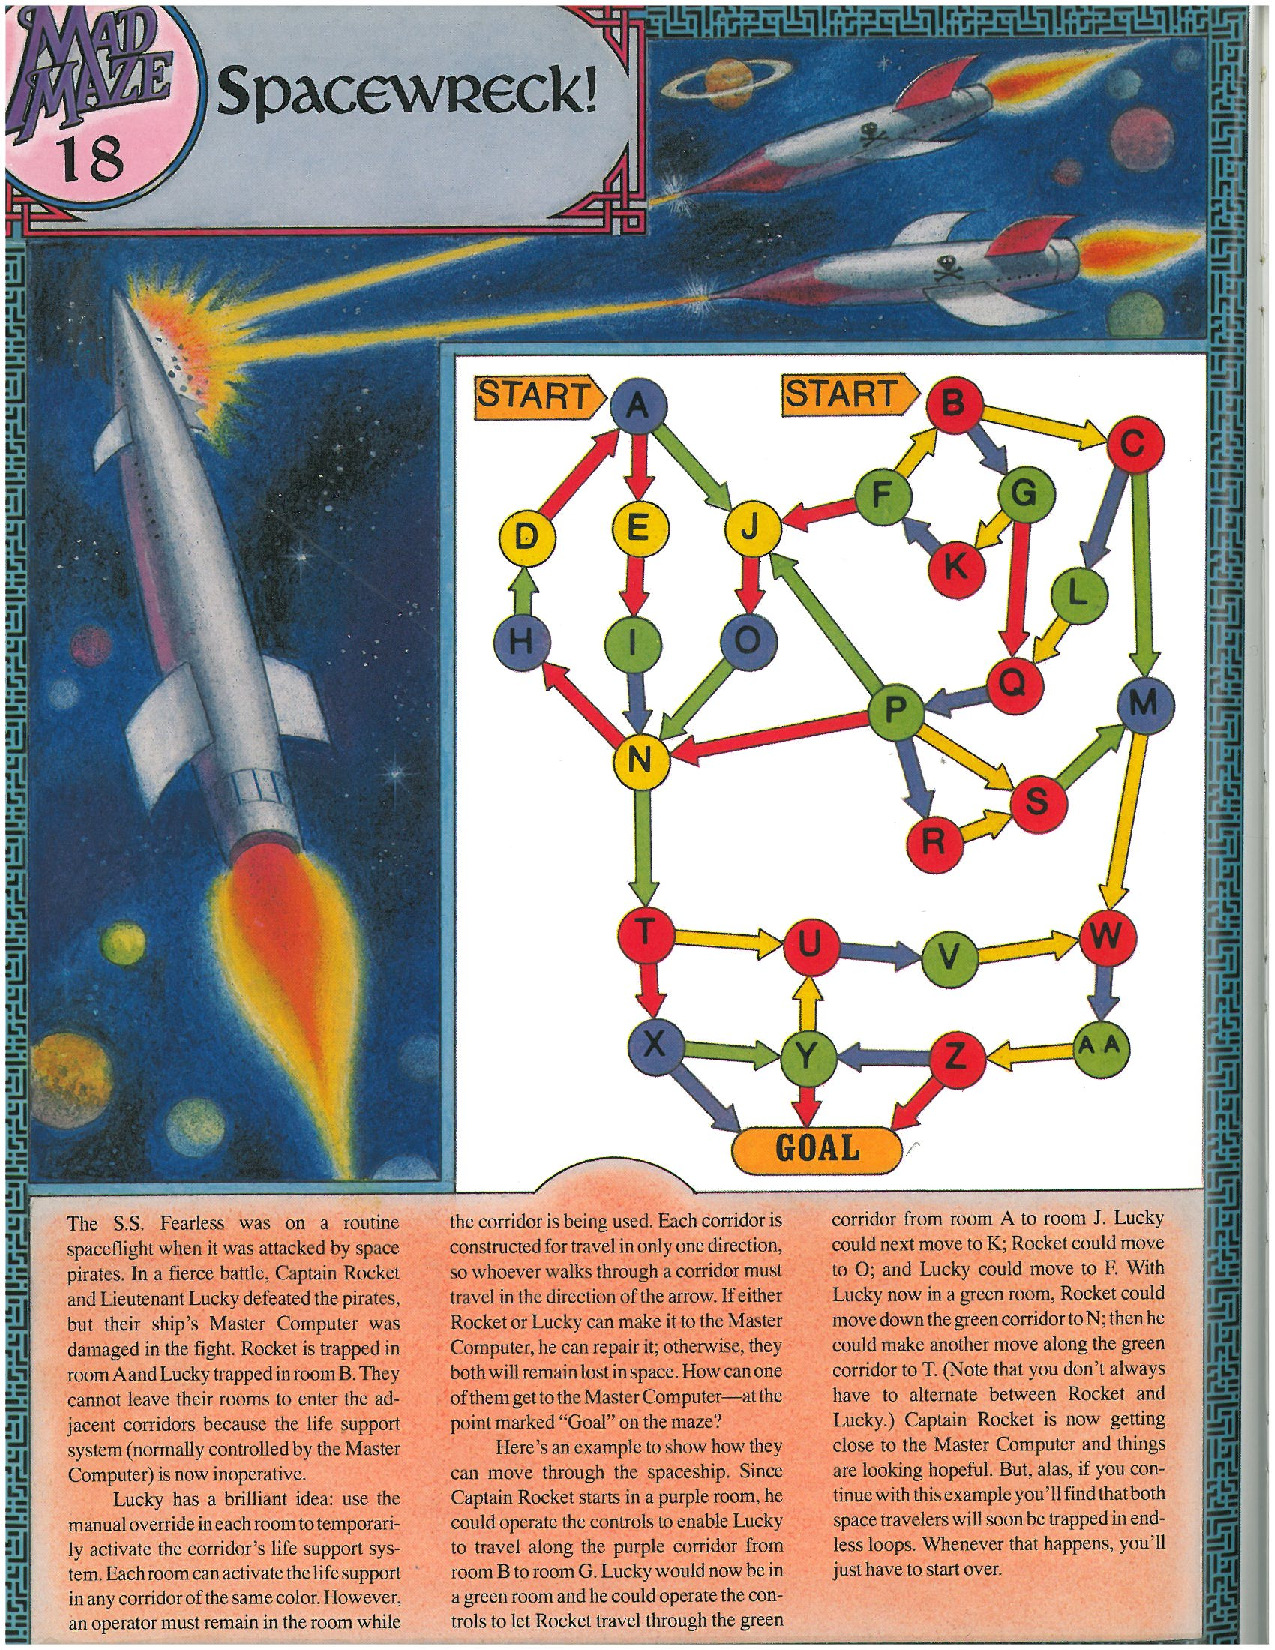
\includegraphics[width=0.95\textwidth]{../18SpaceWreck.pdf}
\end{figure}

\pagebreak
\section*{Appendix B: Python Code}
\lstinputlisting[language=Python]{../main.py}



\end{document}
